%%%%%%%%%%%%%%%%%%%%%%%%%%%%%%%%%%%%%%%%%
% Vertical Line Title Page 
% LaTeX Template
% Version 1.0 (27/12/12)
%
% This template has been downloaded from:
% http://www.LaTeXTemplates.com
%
% Original author:
% Peter Wilson (herries.press@earthlink.net)
%
% License:
% CC BY-NC-SA 3.0 (http://creativecommons.org/licenses/by-nc-sa/3.0/)
% 
% Instructions for using this template:
% This title page compiles as is. If you wish to include this title page in 
% another document, you will need to copy everything before 
% \begin{document} into the preamble of your document. The title page is
% then included using \titleGM within your document.
%
%%%%%%%%%%%%%%%%%%%%%%%%%%%%%%%%%%%%%%%%%

%----------------------------------------------------------------------------------------
%	PACKAGES AND OTHER DOCUMENT CONFIGURATIONS
%----------------------------------------------------------------------------------------

\documentclass{article}

\usepackage[utf8]{inputenc}

\usepackage{xcolor}
\usepackage{listings}
\usepackage{epsfig}
\usepackage{graphics, float}
\usepackage{color, soul}
\usepackage[ampersand]{easylist}

\usepackage{amsmath}

\DeclareMathOperator{\deriv}{d}

\newcommand*{\plogo}{\fbox{$\mathcal{PL}$}} % Generic publisher logo
\newcommand{\hlc}[2][yellow]{ {\sethlcolor{#1} \hl{#2}} }

\ListProperties(Hide=100, Hang=true, Progressive=3ex, Style*=-- , % custom listing
Style2*=$\bullet$ ,Style3*=$\circ$ ,Style4*=\tiny$\blacksquare$ )

%----------------------------------------------------------------------------------------
%	TITLE PAGE
%----------------------------------------------------------------------------------------

\newcommand*{\titleGM}{\begingroup % Create the command for including the title page in the document
\hbox{ % Horizontal box
	\hspace*{0.2\textwidth} % Whitespace to the left of the title page
	\rule{1pt}{\textheight} % Vertical line
	\hspace*{0.05\textwidth} % Whitespace between the vertical line and title page text
	\parbox[b]{0.85\textwidth}{ % Paragraph box which restricts text to less than the width of the page
		
		{\noindent\Huge\bfseries Super Neural Network }\\[2\baselineskip] % Title
		{\large \textit{Laboratório de Circuitos Digitais \\ Turma B, Grupo 13}}\\[4\baselineskip] % Tagline or further description
		{\Large \textsc{Isadora Sophia e Matheus Diamantino} \\} % Author name
        {\textsc{RA 158018 e RA 156740} \\ \\} % RAs
        {\textsc{isaecia@gmail.com \\ matdiamantino@gmail.com}\\} % emails
		
		\vspace{0.5\textheight} % Whitespace between the title block and the publisher

        {\small{22 de Junho de 2016}}
		%{\noindent The Publisher \plogo}\\[\baselineskip] % Publisher and logo
	}}
	\endgroup}

\newcommand{\colorbitbox}[3]{%
	\rlap{\bitbox{#2}{\color{#1}\rule{\width}{\height}}}%
	\bitbox{#2}{#3}}

%----------------------------------------------------------------------------------------
%	BLANK DOCUMENT
%----------------------------------------------------------------------------------------

\begin{document}

\pagestyle{empty} % Removes page numbers

\titleGM % This command includes the title page

\section{Introdução} \label{sec:int}
Redes neurais são modelos probabilísticos propostos a partir do aprendizado com a \textbf{experiência}. Isto é, iterações são feitas em um modelo de dados de forma a adequar a estrutura para um padrão de saída específico.

O trabalho final de circuitos digitais se baseia na implementação de uma rede neural em FPGA, utilizando VHDL. Também foi utilizado um display de VGA, para disponibilizar a saída de uma forma mais visual ao usuário.

\section{Teoria} \label{sec:int}
    \subsection{Redes neurais}
        Redes neurais tratam-se de um modelo composto por uma estrutura de \textbf{neurônios}, separados em \textit{layers}, com função de prever uma saída para cada entrada recebida.

        \subsubsection{Feedforward}
            \textit{Feedforward} se baseia na operação de calcular a saída, dada uma entrada e uma estrutura já pré-definida da rede. No caso, cada neurônio possui um valor de ativação, chamado de $a^{(i)}_j$, com $i =$ layer do neurônio e $j =$ neurônio correspondente, que corresponde ao `output' de cada neurônio.

            Por exemplo, para a layer 1 (\textit{input}), o vetor $a^{(1)}$ corresponde simplesmente à entrada - enquanto para a layer 3 (na figura), o vetor $a^{(3)}$ corresponde ao output.

            \begin{figure}[ht!]
              \centering
              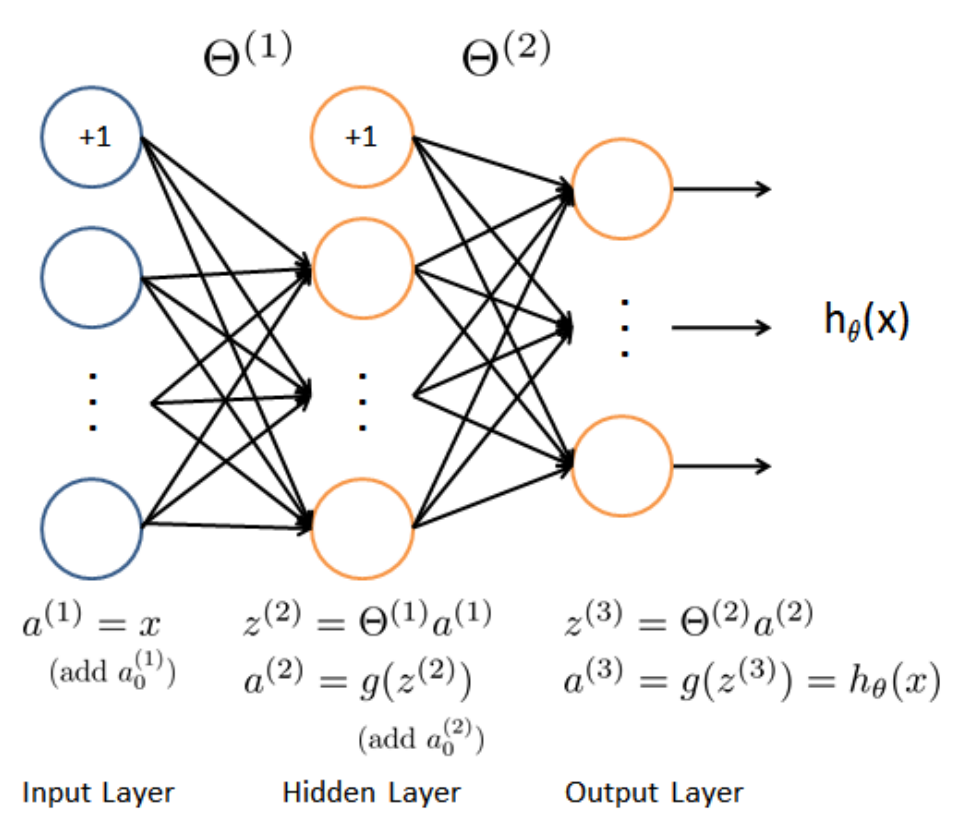
\includegraphics[width=7cm]{figures/nn_model}
              \caption{Exemplo de rede neural de três layers, retirado de \cite{MLC}}
              \label{fig:arch}
            \end{figure}

            A geração do valor de ativação depende das \textbf{entradas} e \textbf{pesos} da rede. Em cada neurônio, as entradas correspondem ao valor de ativação dos neurônios da layer anterior, multiplicado pelo seu respectivo peso. 

            Os pesos são representados, tipicamente, por uma matriz $\Theta^{(i)}$, com $i =$ layer correspondente, em que cada $w_{ij}$ representa o peso da entrada $i$ para o neurônio $j$.

            Assim, cada neurônio computa $z^{(i)}_j$, $i =$ layer do neurônio e $j =$ neurônio correspondente, que é a soma da multiplicação dos pesos e dos valores de ativação. Finalmente, para que o valor possa convergir para $0$ ou $1$, é aplicada uma função $g(x)$, correspondente à função \textit{sigmoid}. Logo, $g(z^{(i)}_j) = a^{(i)}_j$.

            A operação em que a rede neural calcula a resposta a partir dos pesos em $\Theta^{(i)}$ é chamada na literatura de feedforward. 

        \subsubsection{Backpropagation}
            Para que uma rede neural realize a validação dos resultados, é necessário estabelecer a \textit{backpropagation}, que corresponde à operação de treinamento. Note que essa operação é realizada apenas se a rede neural estiver na função de \textbf{aprendizado}.

            \begin{figure}[ht!]
              \centering
              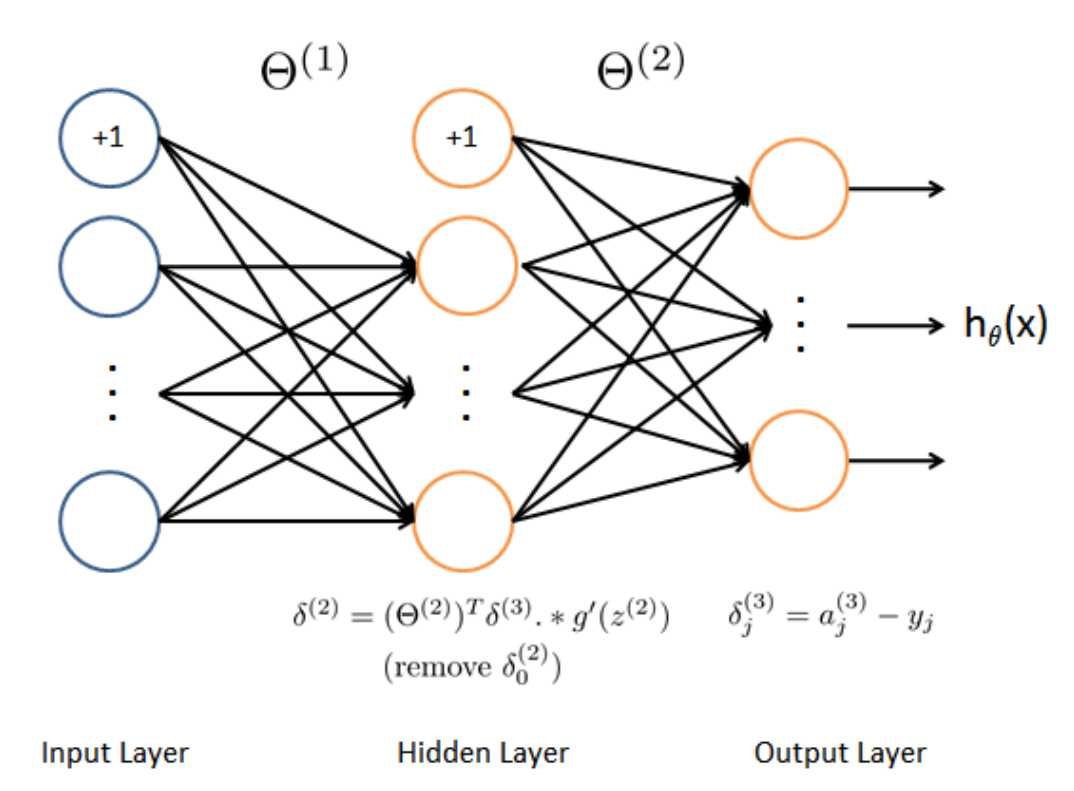
\includegraphics[width=9cm]{figures/nn_model_back}
              \caption{Exemplo de rede neural de três layers, retirado de \cite{MLC}}
              \label{fig:arch}
            \end{figure}

            É necessário que a rede neural valide a saída atual a partir da saída ideal, uma vez que ela está sendo treinada a partir de um banco de dados de treinamento, com entradas e saídas corretas. Assim, é calculado um $\delta^{(i)}_k$, em que $i =$ layer do neurônio e $k =$ layer correspondente, que equivale à margem de erro encontrada no resultado.

            O mais importante dessa etapa é a \textbf{propagação} do erro para as demais layers. Assim, o $\delta^{(3)}_k$, que seria da saída, corresponde a:

            \begin{equation}
                \delta^{(3)}_k = a^{(3)}_k - y_k
            \end{equation}

            Sendo $y_k$ a saída correta da entrada para o neurônio $k$. Os demais valores de $\delta^{(i)}_k$ devem seguir a seguinte equação:

            \begin{equation}
                \delta^{(i)}_k = \left(\sum_{j = 1}^O \Theta^{(i)}_{kj} \cdot \delta^{(i + 1)}_{j}\right) \cdot \cfrac{\deriv g(z^{(i)}_k)}{\deriv z}
            \end{equation}

            Note que o valor de \textit{bias}, que equivale ao valor de $\delta^{(i)}_0 = 1$ em cada uma das layers, não é aplicado nas operações anteriores. Ele deve ser utilizado para essa última etapa. Finalmente, obtém-se o valor final da propagação de erros para cada peso $w_{ij}$, para cada $\Theta^{(i)}$:

            \begin{equation}
                \Delta^{(l)}_{ij} = a^{(l)}_i \cdot \delta^{(l + 1)}_j
            \end{equation}

            Agora, para que cada peso seja atualizado adequadamente, a operação é realizada:

            \begin{equation}
                w^{(l)}_{ij} = w^{(l)}_{ij} - (\lambda \cdot \Delta^{(l)}_{ij})
            \end{equation}

            Em que $\lambda$ corresponde ao \textit{learning rate} da rede neural. Finalmente, a operação de backpropagation está concluída. O ideal é que ela realize diversas iterações até que os pesos estejam adequados para a operação realizada.

    \subsection{Sigmoid}
        A função \textit{sigmoid} foi a função escolhida para estimar os valores de saída entre $0$ e $1$. Foram seguidas referências de literatura para a escolha dessa função (bastante utilizada em redes neurais), que é dada por:

        \begin{equation}
            g(x) = \cfrac{1}{1 + e^{-x}}
        \end{equation}

        Os valores de saída são apresentados na gravura abaixo.

        \begin{figure}[ht!]
          \centering
          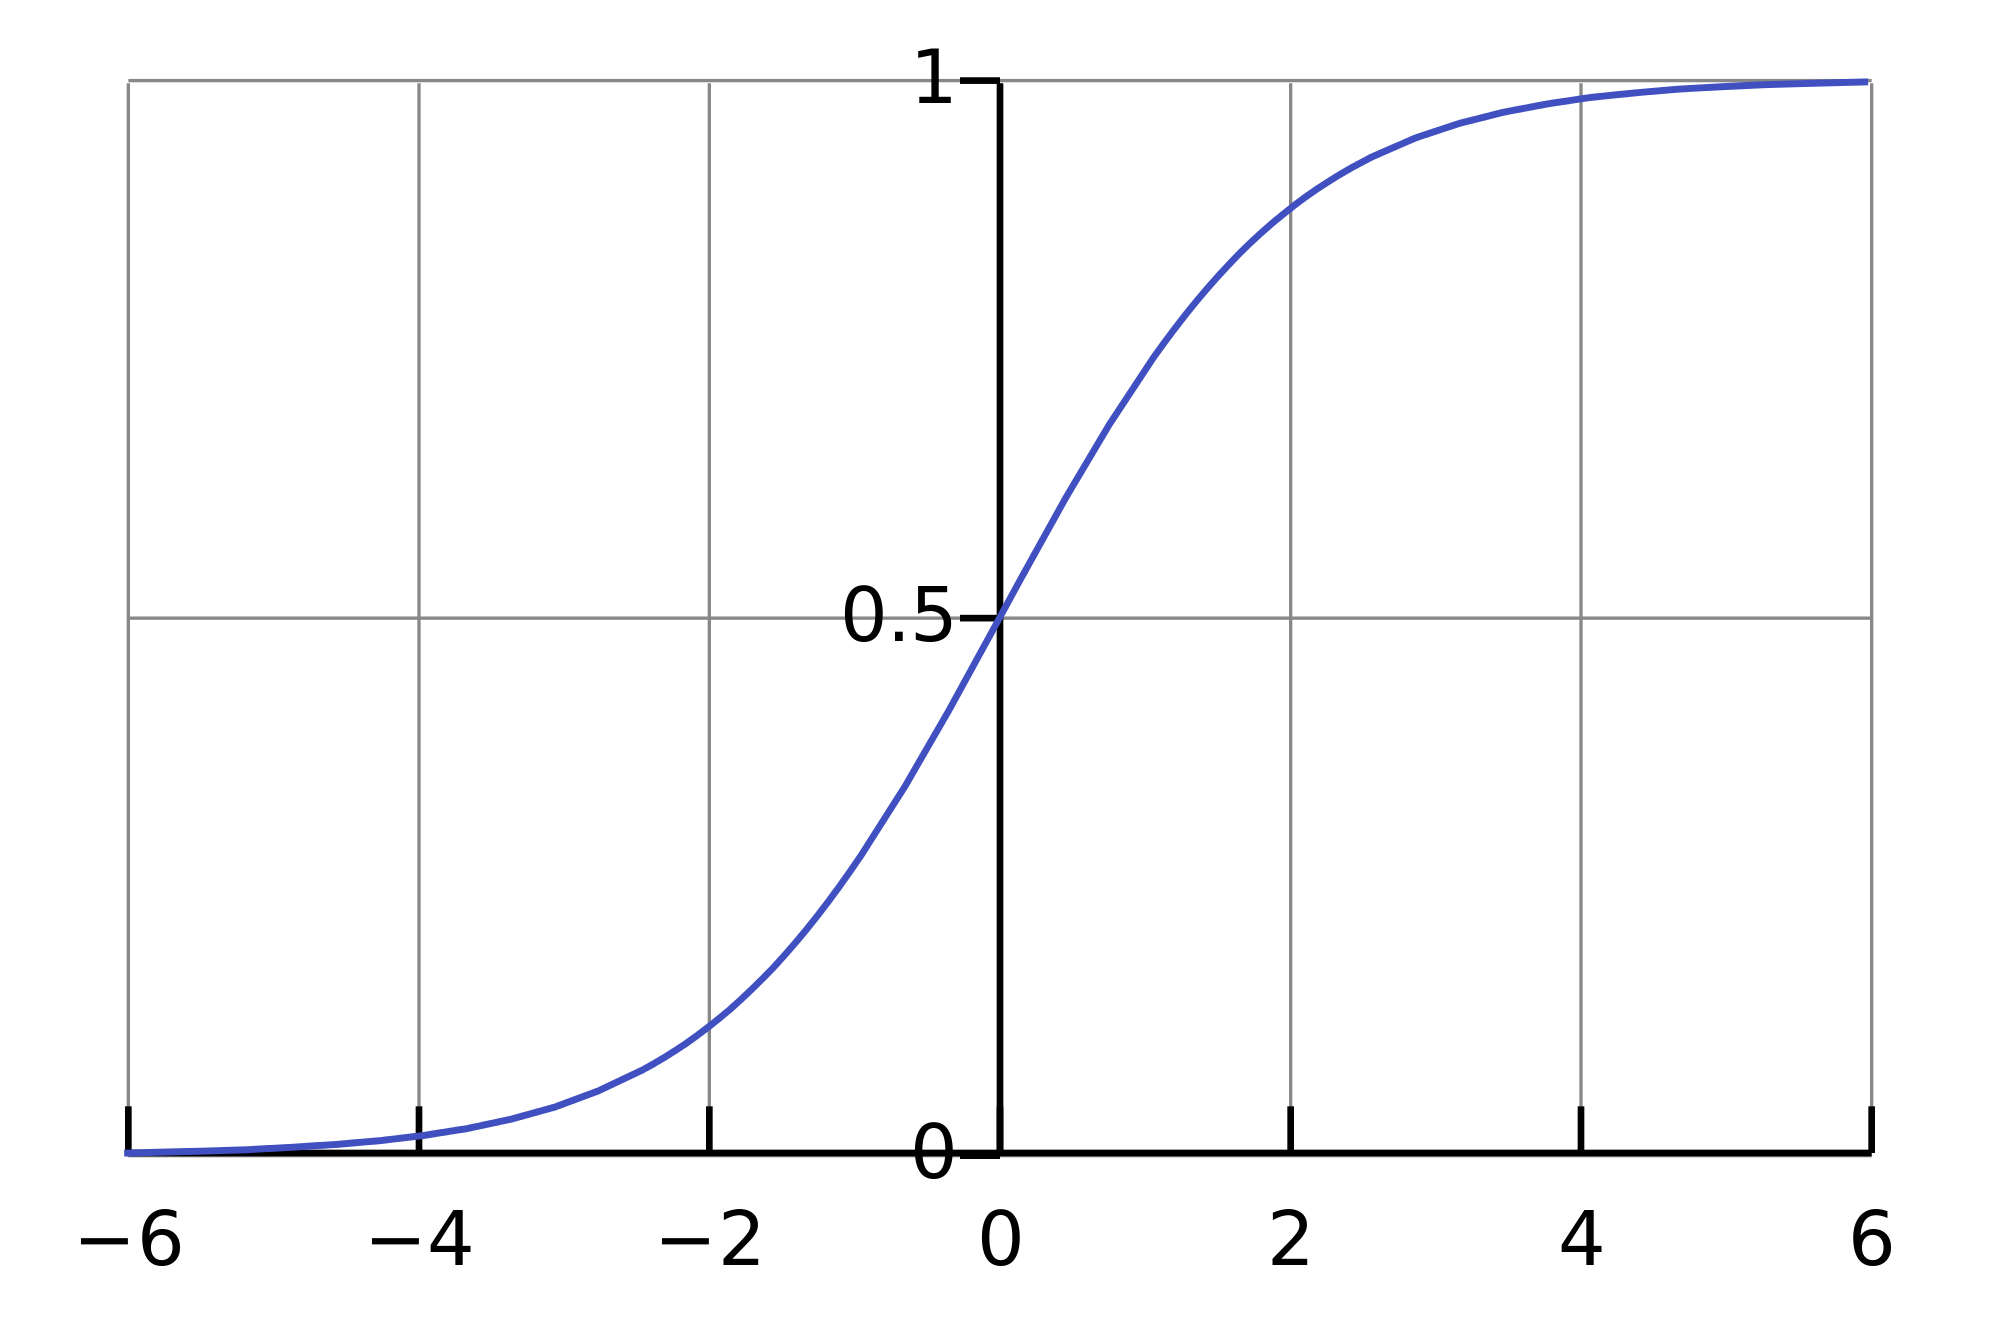
\includegraphics[width=6cm]{figures/sigmoid}
          \caption{Função sigmoid}
          \label{fig:arch}
        \end{figure}


\section{Descrição do sistema}
    A implementação do sistema se baseava na seguinte estrutura:

    \begin{figure}[ht!]
      \centering
      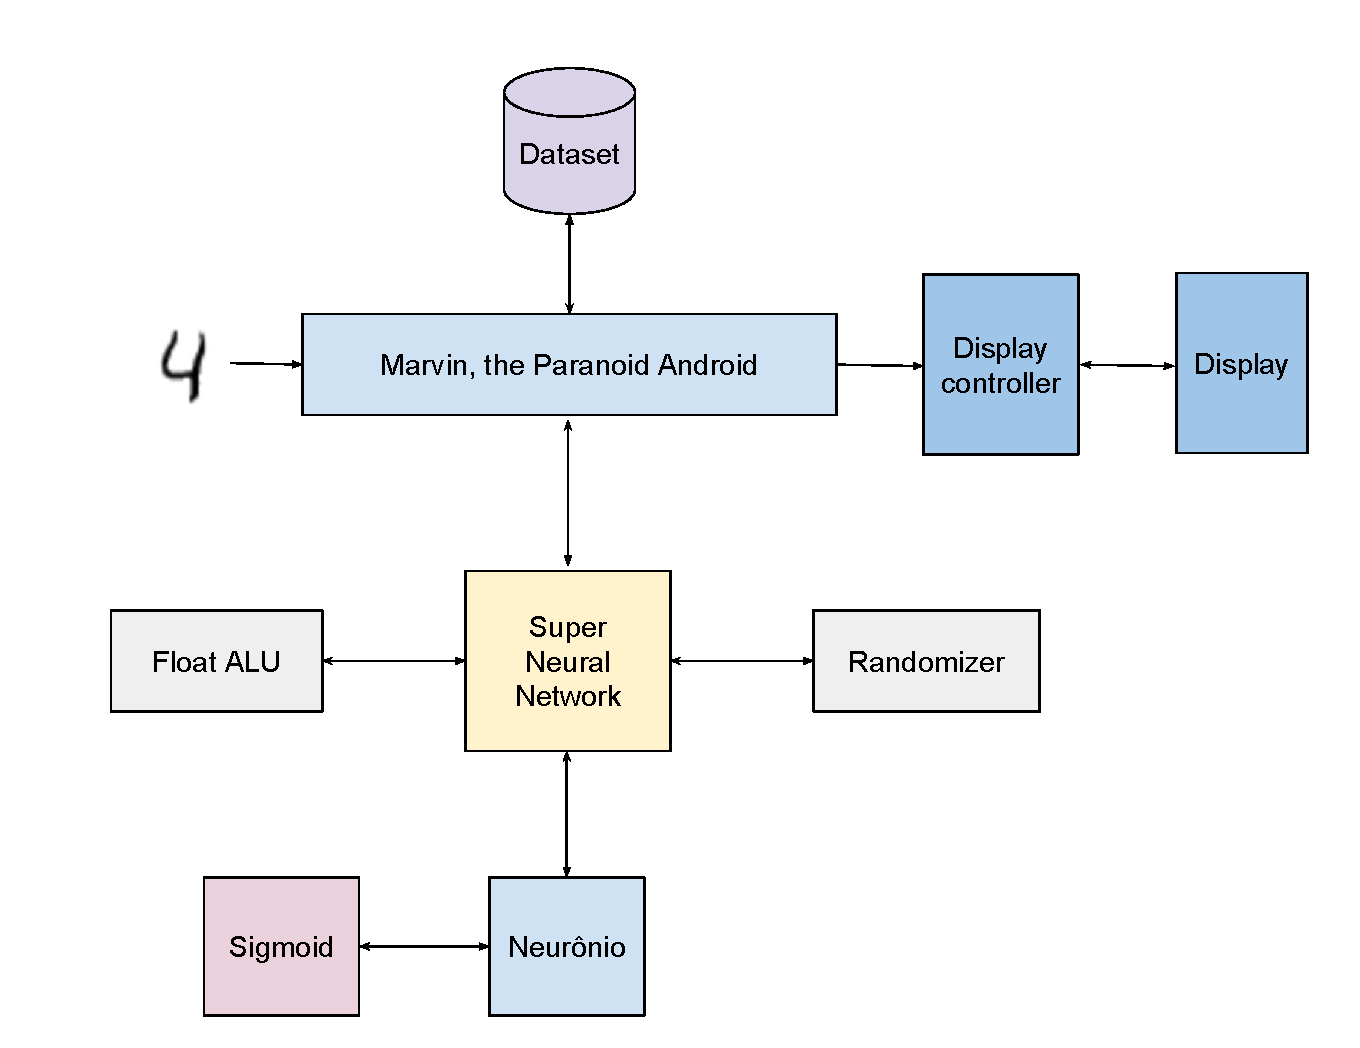
\includegraphics[width=12cm]{figures/blk_d}
      \caption{Diagrama de blocos do projeto}
      \label{fig:arch}
    \end{figure}

    \subsection{Estrutura do projeto}

    Inicialmente, o trabalho consistiria na identificação de dígitos de $0$ a $9$, utilizando o banco de dados \textbf{MNIST} para o treinamento da rede neural. Cada imagem do banco de dados tem $20$x$20$ pixels, constituídos de pixels da escala cinza.

    \begin{figure}[ht!]
      \centering
      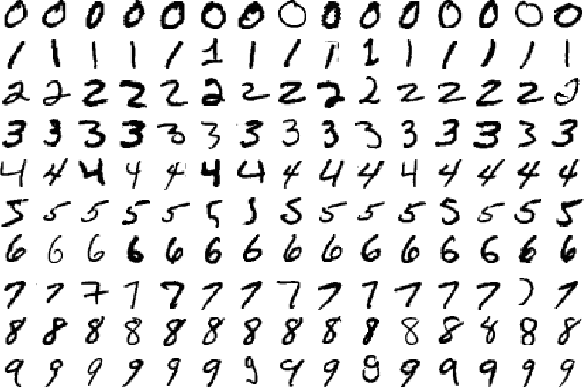
\includegraphics[width=6.5cm]{figures/mnistdigits}
      \caption{MNIST dataset}
      \label{fig:arch}
    \end{figure}

    Para que a identificação de dígitos pudesse ser realizada, o modelo de rede neural foi simulado em \textit{Octave}: seriam necessários $400$ neurônios como entrada na layer 1, $25$ neurônios na layer 2 e $10$ neurônios como saída na layer 3. 

    Ou seja, apenas na layer 2, seriam necessários: $25 \cdot 400 \cdot 400p$ bits reservados na placa, com $p =$ precisão que seria utilizada nos valores. Diante da quantidade de memória necessária, foi implementado um componente de \textbf{SRAM}.

    Inicialmente, foi implementada uma SRAM assíncrona. Como o resultado não foi conforme o esperado, a SRAM foi reimplementada de forma síncrona. O número de palavras assignado foi de 256k, com cada palavra de 16 bits.

    Entretanto, ao realizar testes com a SRAM, o grupo estabeleceu que a implementação de uma rede neural (que precisava, antes de tudo, ser validada) utilizando sistemas complexos com largas quantidades de memória não era viável para o trabalho, pelo menos em primeiro plano. Diante disso, a utilização do banco de dados MNIST e a SRAM foram deixados de lado. 

    Logo, para validar o funcionamento completo da rede neural, foi convecionado o treinamento de funções lógicas, como a \textbf{XOR}. Esta validação foi escolhida uma vez que é amplamente utilizada pela comunidade para validar o funcionamento de um determinado modelo probabilístico.

    \begin{figure}[ht!]
      \centering
      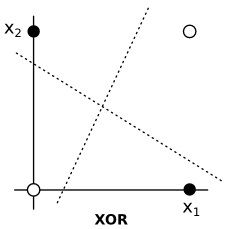
\includegraphics[width=4cm]{figures/xor-plot}
      \caption{Gráfico da função XOR, o qual não pode ser aproximado por uma função linear}
      \label{fig:arch}
    \end{figure}

    \subsection{Questões técnicas}
    Em seguida, foi estabelecida a precisão que seria utilizada nos valores. Por questões práticas, foi estabelecido utilizar \textbf{fixed point representation} para realizar as contas. Foi implementada uma \textbf{ALU} para lidar com as contas e as demais flags relacionadas a operações aritméticas.

    Diante do desafio de implementar uma ALU completa, foi encontrado um \textit{fixed\_pkg} do ieee com uma implementação robusta de fixed point, e decidimos incorporá-la ao trabalho. Assim, utilizamos uma ALU e o fixed\_pkg para realizar as contas com fixed point, com tamanho de 16 bits (8 casas inteiras e 8 decimais).

    Um último aspecto que precisava ser discutido era relacionado à função \textbf{sigmoid}. Consultamos diversos papers na literatura em relação à implementação da função sigmoid de forma eficiente, sem envolver exponenciação ou complicações.

    Decidimos que a forma mais eficiente e precisa seria através de uma implementação por \textsc{lookup table}. Escrevemos um código em C++ para gerar uma lookup table com precisão de 5 casas decimais da sigmoid function, em fixed point. Também foi gerada uma lookup table para a derivada da sigmoid.

    Também utilizamos um divisor de clock (como implementado em laboratórios) para tornar o clock da placa flexível durante os testes.

    \subsection{Implementação dos componentes}
    Começamos implementando as partes com menor acoplamento, para permitir a realização de testes e garantir o funcionamento do componente ao incorporá-lo em partes maiores do projeto. 

    Assim, implementamos um componente simples chamado \textbf{Randomizer}, responsável por criar valores pseudo-randômicos para a inicialização de pesos da rede neural. O componente utiliza do algoritmo de LFSR, em que a seed é alterada a cada borda de clock a partir de uma operação de \textsc{XNOR}, seguido por um \textsc{SHIFT}. Os valores inicializados foram limitados ao intervalo entre 0 e 1, de forma a garantir a integridade do aprendizado da rede neural.

    Em seguida, foi proposto o funcionamento do componente do \textbf{Neurônio}. Basicamente, cada neurônio calcula seu valor de ativação:

    \begin{equation}
        a^{(i)}_j = g\left(\sum_{k = 1}^{n} w_{kj} a^{(i-1)}_k\right)
    \end{equation}

    Bastou-se utilizar a ALU e o componente da sigmoid para a implementação do neurônio. Realizamos alguns testes de valores, traduzimos fixed point para representação decimal e verificamos se os números são compatíveis. A taxa de erro foi de, aproximadamente, $10^{-3}$. Consideramos razoável para o desempenho do treinamento.

    Decidimos prosseguir e testar o \textsc{feedforward}. Para isso, precisaríamos do componente \textbf{Marvin}, the Paranoid Android e \textbf{SNN}, Super Neural Network.

    Marvin fica responsável por receber os inputs do usuário, tratar tais sinais e levá-los ao componente SNN. Temos dois estados, RUNNING e IDLE, que determinam se a rede neural irá processar os dados ou não. O modo IDLE é chamado sempre que o componente é resetado.
    
    Quando estamos no modo RUNNING, este possui dois subestados: Learning e Not Learning, determinados por um input de usuário. Quando o componente está com Learning ativo, o ciclo de clock será dividido em atualizar os novos pesos e receber novos inputs. Quando ele está com Learning desativado, apenas atualizamos os inputs recebidos pelo usuário.

    A partir do Marvin, instanciamos a SNN, que fica responsável por receber os parâmetros e fornecê-los aos neurônios que são instanciados neste componente. No caso específico deste projeto, temos 2 neurônios de entrada, 2 para a hidden layer e 1 para o output.

    Ao constatar o funcionamento do feedforward, prosseguimos para o backpropagation. Primeiramente, foi implemeantado o componente para o \textbf{lower delta output}, que se baseia, como demonstrado anteriormente, em:

    \begin{equation}
        \delta^{(3)}_k = a^{(3)}_k - y_k
    \end{equation}

    Utilizando-se a ALU, bastando receber o $a$ e o $y$. Logo em seguida, foi implementado o \textbf{lower delta hidden}, que faz o seguinte cálculo:

    \begin{equation}
        \delta^{(i)}_k = \left(\sum_{j = 1}^O \Theta^{(i)}_{kj} \cdot \delta^{(i + 1)}_{j}\right) \cdot \cfrac{\deriv g(z^{(i)}_k)}{\deriv z}
    \end{equation}

    O componente recebe como parâmetro todos os \textit{pesos} correspondetes e \textit{deltas} da layer do output, de tamanho $O$. Além disso, deve receber $z^{(i)}_k$, ou seja, do neurônio atual. É utilizado a ALU e a função de derivada da sigmoid.

    Um único componente, \textbf{upper delta}, foi criado para o cálculo de $\Delta$, como:

    \begin{equation}
        \Delta^{(l)}_{ij} = a^{(l)}_i \cdot \delta^{(l + 1)}_j
    \end{equation}

    O qual recebe um valor $a^{(l)}_i$ e $\delta^{(l + 1)}_j$ como parâmetros e os multiplica. Note que o principal propósito desses componentes é garantir a abstração do componente da rede neural e organizar melhor o trabalho de execução. Finalmente, basta-se criar um componente \textbf{new\_weight}, responsável por atualizar os pesos.

    \begin{equation}
        w^{(l)}_{ij} = w^{(l)}_{ij} - (\lambda \cdot \Delta^{(l)}_{ij})
    \end{equation}

    O componente recebe o \textit{peso antigo}, o \textit{learning rate} e $\Delta^{(l)}_{ij}$.

    Assim, o Marvin precisou ser modificado de modo a realizar o backpropagation. Além disso, foi necessário criar um novo componente semelhante ao SNN, \textbf{SNN\_learn}, responsável pelo aprendizado da rede neural e por coordenar todos os parâmetros para cada componente apropriado.

    O SNN\_learn é responsável por receber a saída atual do feedforward e os parâmetros necessários para o cálculo dos erros para minimizar a função. Para isso, são instanciados os componentes  \textbf{lower delta hidden}, \textbf{lower delta output} e \textbf{upper delta}.

    Com este novo componente, foi possível instanciá-lo no Marvin para o cálculo dos erros com o componente \textbf{new\_weight}. Deste modo, quando estamos com Learning ativo, foi possível atualizar os pesos antigos e, assim, realizar a operação de aprendizado.

    Assim que o projeto parecia estar em ordem, foi iniciado a etapa de testes. Os principais desafios envolveram escolher valores dos pesos inicias e o valor do learning rate, que afetava significativamente o resultado do aprendizado da rede. Em algumas tentativas, o erro era tão grande que a dúvida restava era se o código estava correto (principalmente em respeito aos componentes SNN e SNN\_learn), e refizemos os componentes cerca de três vezes, até constatar que o erro estava, de fato, nos valores dos parâmetros.

    As simulações no Quartus se mostraram extremamente lentas e a simulação na própria placa foi a forma mais eficiente de averiguar o desempenho da estrutura. Após diversas análises, fixamos um valor pra a learning rate de $\lambda = 0.05$ e pesos iniciais para valores entre $0$ e $1$. A rede neural estava aprendendo corretamente as operações lógicas de XOR, AND, OR e XNOR.

    Com o projeto próximo da conclusão, prosseguimos incluindo switches para o usuário escolher a função lógica para treinar a rede neural (XOR, AND, OR e XNOR) - basta setar o switch e treinar a placa para que ela passe a realizar a operação. Em nossa nomenclatura:

    \begin{itemize}
        \item \textbf{00} = XOR
        \item \textbf{01} = AND
        \item \textbf{10} = OR
        \item \textbf{11} = XNOR
    \end{itemize}

    Procuramos, também, aproximar essa solução de uma forma como a sugerida pelo professor Cortes, em que a rede neural passaria a ter 4 inputs e identificaria a operação lógica automaticamente - em que os dois primeiros bits corresponderiam aos inputs em si, e os bits restantes seriam a representação da operação lógica a ser utilizada. Por exemplo, a entrada \textbf{0100} representa a operação entre 0 e 1, dado que a operação lógica tem código \textbf{00} (que, no nosso caso, seria um XOR). Entretanto, não foi possível concluir um treinamento eficiente com esse modelo, composto por 4 inputs e 4 neurônios na hidden layer, devido a valores incorretos de $\lambda$, além de alguns parâmetros que resultavam em overflow e em um comportamento anômalo da placa. 

    Resolvemos lidar com esse problema a partir da implementação citada anteriormente, de switches que definem a operação lógica a ser aprendida, uma vez que se apresentou como uma forma mais simples.

    Finalmente, acrescentamos a implementação do display de VGA. Utilizamos os componentes \textbf{OutputDriver} e \textbf{vgacon} do grupo 2, de Leonardo Villani e Thiago Silva (Tetris). Foi implementada uma simples amostragem de dados, ou seja, mostra-se os pesos ($\Theta^{(1)}$ e $\Theta^{(2)}$, em fixed point) e o resultado do output final (0 ou 1).

\section{Conclusão}
    O projeto foi de muita importância para um aprendizado mais amplo e aprofundado em relação ao comportamento da FPGA e da linguagem de VHDL. Foi estabelecida a importância de ferramentas de debug, isto é, formas de acompanhar os resultados e entender o procedimento que ocorre na placa - uma vez que isso economizaria várias horas de simulação e detecção de erros, se investidas de forma mais aprofundada.

    O projeto final, por fim, concluiu-se da seguinte forma:

   \begin{figure}[ht!]
      \centering
      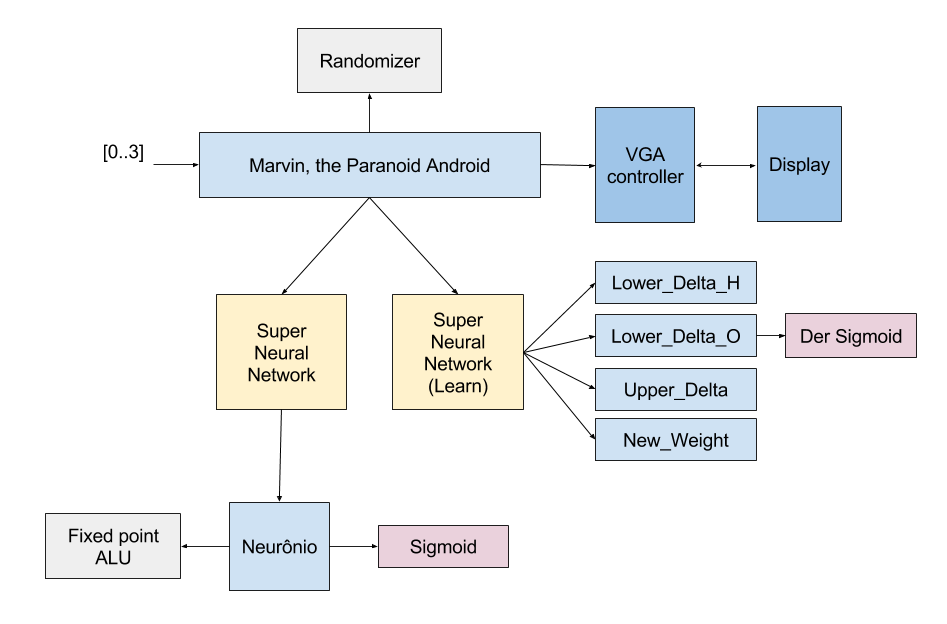
\includegraphics[width=13cm]{figures/blk_d_new}
      \caption{Diagrama de blocos final} 
      \label{fig:arch}
    \end{figure}

\bibliography{bib/tasklab} 
\bibliographystyle{ieeetr}

\end{document}
